\documentclass[11pt,a4paper,twoside,openright]{report}

\usepackage[top=25mm,bottom=25mm,right=25mm,left=30mm,head=12.5mm,foot=12.5mm]{geometry}
\let\openright=\cleardoublepage

\usepackage[a-2u]{pdfx}

\usepackage[
   backend=biber
  ,style=iso-authoryear
  ,style=numeric
  ,citestyle=numeric
  ,sortlocale=cs_CZ
  ,bibencoding=UTF8
  ,block=ragged
]{biblatex}
\addbibresource{references.bib}



%% Přepneme na českou sazbu, fonty Latin Modern a kódování češtiny
\usepackage[english]{babel}
\usepackage{lmodern}
\usepackage[T1]{fontenc}
\usepackage{textcomp}
\usepackage[utf8]{inputenc}

\usepackage{amssymb}
%%% Set the times symobl to be a dot instad of a star
\DeclareMathSymbol{*}{\mathbin}{symbols}{"01}
% Set fonts
\RequirePackage[osf]{mathpazo} % Palatino with oldstyle figures
\newcommand\liningnums[1]{\fontfamily{ppl}\selectfont#1}
\RequirePackage{eulervm}
\RequirePackage[scaled=.8819]{sourcecodepro} % Source Code Pro typeface for monospace

%%% Další užitečné balíčky (jsou součástí běžných distribucí LaTeXu)
\usepackage{amsmath}        % rozšíření pro sazbu matematiky
\usepackage{amsfonts}       % matematické fonty
\usepackage{amsthm}         % sazba vět, definic apod.
\usepackage{bm}             % tučné symboly (příkaz \bm)
\usepackage{graphicx}       % vkládání obrázků
\usepackage{fancyvrb}       % vylepšené prostředí pro strojové písmo
\usepackage{fancyhdr}       % prostředí pohodlnější nastavení hlavy a paty stránek
\usepackage{icomma}         % inteligetní čárka v matematickém módu
\usepackage{dcolumn}        % lepší zarovnání sloupců v tabulkách
\usepackage{booktabs}       % lepší vodorovné linky v tabulkách
\makeatletter
\@ifpackageloaded{xcolor}{
   \@ifpackagewith{xcolor}{usenames}{}{\PassOptionsToPackage{usenames}{xcolor}}
  }{\usepackage[usenames]{xcolor}} % barevná sazba
\makeatother
\usepackage{multicol}       % práce s více sloupci na stránce
\usepackage{caption}
\usepackage{enumitem}
\usepackage{lipsum}
\setlist[itemize]{noitemsep, topsep=0pt, partopsep=0pt}
\setlist[enumerate]{noitemsep, topsep=0pt, partopsep=0pt}
\setlist[description]{noitemsep, topsep=0pt, partopsep=0pt}
\usepackage{pdfpages}

\usepackage{csquotes}


\usepackage{tocloft}
\setlength\cftparskip{0pt}
\setlength\cftbeforechapskip{1.5ex}
\setlength\cftfigindent{0pt}
\setlength\cfttabindent{0pt}
\setlength\cftbeforeloftitleskip{0pt}
\setlength\cftbeforelottitleskip{0pt}
\setlength\cftbeforetoctitleskip{0pt}
\renewcommand{\cftlottitlefont}{\Huge\bfseries}
\renewcommand{\cftloftitlefont}{\Huge\bfseries}
\renewcommand{\cfttoctitlefont}{\Huge\bfseries}

% vyznaceni odstavcu
\parindent=0pt
\parskip=11pt

% zakaz vdov a sirotku - jednoradkovych pocatku ci koncu odstavcu na prechodu mezi strankami
\clubpenalty=1000
\widowpenalty=1000
\displaywidowpenalty=1000

% nastaveni radkovani
\renewcommand{\baselinestretch}{1.20}

% nastavení hlavy a paty stránek
\fancyhf{}
\renewcommand{\chaptermark}[1]{\markboth{#1}{}}
\fancyhead[RO,LE]{\leftmark}
\fancyfoot[RO,LE]{\thepage}
%\renewcommand{\footrulewidth}{0pt}
\fancypagestyle{plain}{%
\fancyhf{} % clear all header and footer fields
\fancyfoot[RO,LE]{\thepage}
\renewcommand{\headrulewidth}{0pt}
%\renewcommand{\footrulewidth}{0.5pt}
}

% Tato makra přesvědčují mírně ošklivým trikem LaTeX, aby hlavičky kapitol
% sázel příčetněji a nevynechával nad nimi spoustu místa. Směle ignorujte.
\makeatletter
\def\@makechapterhead#1{
  {\parindent \z@ \raggedright 
   \Huge\bfseries \thechapter. #1
   \par\nobreak
   \vskip 20\p@
}}
\def\@makeschapterhead#1{
  {\parindent \z@ \raggedright 
   \Huge\bfseries #1
   \par\nobreak
   \vskip 20\p@
}}
\makeatother

% Trochu volnější nastavení dělení slov, než je default.
\lefthyphenmin=2
\righthyphenmin=2

% Zapne černé "slimáky" na koncích řádků, které přetekly, abychom si
% jich lépe všimli.
\overfullrule=1mm

%% Balíček hyperref, kterým jdou vyrábět klikací odkazy v PDF,
%% ale hlavně ho používáme k uložení metadat do PDF (včetně obsahu).
%% Většinu nastavítek přednastaví balíček pdfx.
\hypersetup{unicode}
\hypersetup{breaklinks=true}
\hypersetup{hidelinks}

%%% Packages for keys
\usepackage{tikz}
\usetikzlibrary{shadows}

\newcommand*\keystroke[1]{%
  \tikz[baseline=(key.base)]
    \node[%
      draw,
      fill=white,
      drop shadow={shadow xshift=0.25ex,shadow yshift=-0.25ex,fill=black,opacity=0.75},
      rectangle,
      rounded corners=2pt,
      inner sep=2pt,
      line width=0.5pt,
      font=\scriptsize\sffamily
    ](key) {\:#1\strut\:}
  ;
}

%%% Prostředí pro sazbu kódu, případně vstupu/výstupu počítačových
%%% programů. (Vyžaduje balíček fancyvrb -- fancy verbatim.)

\DefineVerbatimEnvironment{code}{Verbatim}{fontsize=\small, frame=single}



\def\NazevPrace{Visualizing The Relationship Between Quadratic Julia Sets And Quadratic Mandelbrot Sets}
\def\Trida{4.A}
\def\AutorPrace{Mikuláš Vanoušek}
\def\DatumOdevzdani{2021}

% Vedoucí práce: Jméno a příjmení s~tituly
\def\Vedouci{Šimon Schierreich}

% Studijní program a obor
\def\StudijniProgram{studijní program}
\def\StudijniObor{studijní obor}

% Text čestného prohlášení
\def\Prohlaseni{I hereby declare that the thesis submitted is my unaided work. All direct or indirect
sources used are acknowledged as references.
I am aware that the thesis in digital form can be examined for the use of unauthorized aid
and in order to determine whether the thesis as a whole or parts incorporated in it may be
deemed as plagiarism. For the comparison of my work with existing sources, I agree that it
shall be entered in a database where it shall also remain after examination, to enable
comparison with future theses submitted. Further rights of reproduction and usage, however,
are not granted here.
This paper was not previously presented to another examination board and has not been
published.}

% Text poděkování
\def\Podekovani{%
I would hereby like to thank my thesis advisor Šimon Schierreich for all the advice he has provided. I would like to thank Jaroslav Žukov for his help. Last but not least I would like to express immense gratitude towards Pavel Vanoušek and Iva Vanoušková, who had given me the expensive gift of life and provided me with the environment and support that has allowed me to write this thesis.
}

% Abstrakt česky
\def\Abstrakt{%
Kvadratické Julia sety a kvadratické Mandelbrot sety jsou na sebe kolmé průřezy funkce s dvěma komplexními parametry. Představit si, jak spolu souvisí může být velmi obtížné. Má práce si klade za úkol vizualizovat jejich vztah.
}

% Abstrakt anglicky
\def\AbstraktEN{%
Quadratic Julia sets and quadratic Mandelbrot sets are orthogonal cross-sections of one function with two complex parameters. It can be hard to grasp how exactly those two are related. My thesis aims to visualize the connection and help people understand how Julia sets and Mandelbrot sets are related. 
}

% 3 až 5 klíčových slov
\def\KlicovaSlova{Mandelbrot set, Julia set, Komplexní analýza, OpenGL, vykreslování fraktálů}
% 3 až 5 klíčových slov anglicky
\def\KlicovaSlovaEN{Mandelbrot set, Julia set, Complex Analysis, OpenGL, Fractal rendering}


\begin{document}

%%% Titulní strana práce a další povinné informační strany

%%% Titulní strana práce

\pagestyle{empty}
\pagenumbering{gobble}
\hypersetup{pageanchor=false}

\begin{center}
\LARGE
\textbf{GYMNASIUM JANA KEPLERA}\\
{\large Parléřova 2/118, 169 00 Praha 6}

\vspace{\stretch{3}}


\includegraphics[width=.3\textwidth]{img/logo}

\vspace{\stretch{3}}

{\Huge\bfseries\NazevPrace}

\vspace{8mm}
\mdseries{High school graduation thesis}

\vspace{\stretch{8}}
\large
\begin{tabular}{rl}
Author: & \AutorPrace \\
\noalign{\vspace{2mm}}
Class: & \Trida\\
\noalign{\vspace{2mm}}
School year: & 2020/2021\\
\noalign{\vspace{2mm}}
Subject: & Informatics \\
\noalign{\vspace{2mm}}
Thesis supervisor: & \Vedouci \\
\end{tabular}

\vspace{20mm}
Prague, \DatumOdevzdani
\end{center}


\openright

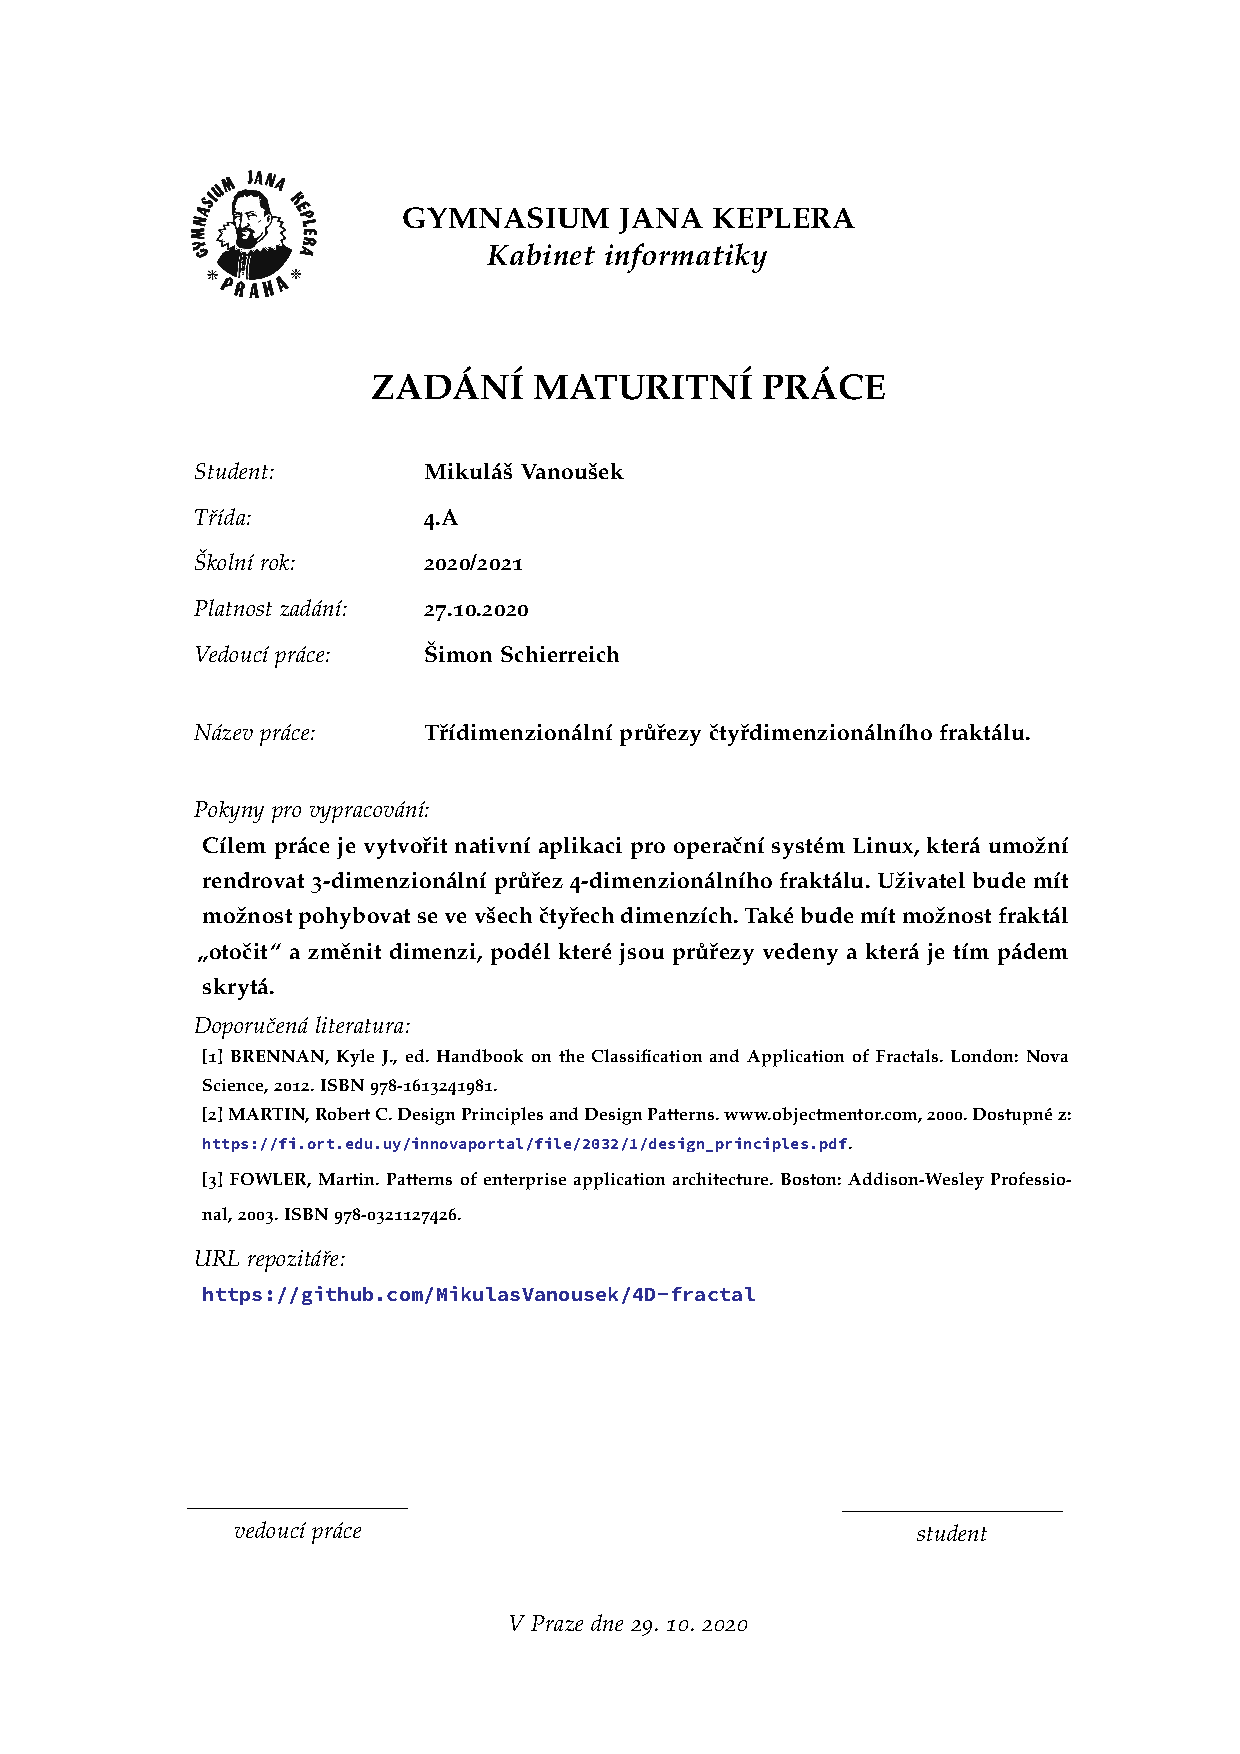
\includepdf[]{zadani.pdf}


%%% Strana s čestným prohlášením k bakalářské práci

\hypersetup{pageanchor=true}
\cleardoublepage
\vspace*{\fill}
\section*{Authorship Declaration}
\noindent
\Prohlaseni

\vspace{2cm}
\noindent
In Prague, \today
\hspace*{\fill}\small{\AutorPrace}
\vspace{1cm}

%%% Poděkování
\openright
\vspace*{\fill}
\section*{Acknowledgements}
\noindent
\Podekovani
\vspace{1cm}


%%% Povinná informační strana bakalářské práce
\openright
\section*{Abstrakt}
\noindent
\Abstrakt
\subsection*{Klíčová slova}
\noindent
\KlicovaSlova

\bigskip\bigskip\bigskip
\section*{Abstract}
\noindent
\AbstraktEN
\subsection*{Keywords}
\noindent
\KlicovaSlovaEN

\openright
\pagenumbering{arabic}

% Obsah
\setcounter{tocdepth}{2}
\tableofcontents

\chapter{Theoretical part}
\pagestyle{fancy}
In the first chapter of my thesis, I will lay down the theoretical foundations of my thesis. I will explain what Mandelbrot sets and Julia sets are, how we can visualize them, how they are part of one 4-dimensional object and how we can visualize this relationship. 

\section{Complex analysis}
Complex analysis investigates the behavior of functions with complex parameters and complex values. The function in question is:
\[f(z, c) = z^n + c\]
\[z,\ c,\ f(z,c) \in \mathbb{C}\]
For given $z$, $c$ we study the behaviour of this function, as it is iterated infinitely many times.
\[z_{0} = z\]
\[z_{n+1} = f(z_n, c)\]
\[F(z, c) = z_{\infty} = \lim_{n\to\infty} z_n\]
For some $z$, $c$ the value of $F(z,\:c)$ is bounded.
\[F(z,c) < k \]
\[ k \in \mathbb{R}\]
For other $z$, $c$ the value of $F(z,\:c)$ is unbounded - it escapes to infinity.
\[F(z,c)     = \infty \]
For unbounded $F(z,c)$ we measure how fast they are growing with the function $g(z,\:c) \in [0;1]$. \cite{complex_analysis}
\section{Approximating $F(z,\:c)$}
A way of computing exact value of $F(z, c)$ for arbitrary $z,c$ has not been found. We have to approximate it. We choose a number of maximum iterations $I_m$ and some escape radius $r\gg0$. Then we iterate the function $f(z,c)$ $i$-times, until one of these conditions is met:
\begin{itemize}
    \item $i = I_m$ - we approximate $F(z,c)$ to be bounded.
    \item $|z_i| > r$ - we approximate $F(z,c)$ to be unbounded and $g(z, c)$ is approximated some function $g'(i, I_m)$.
\end{itemize}

\section{Visualizing complex functions}
On an image with resolution $R_x, R_Y$, we can associate a pixel with $n$ pixels before it in the horizontal direction and $m$ pixels before it in the vertical direction (origin on the bottom left) with a pair of Cartesian coordinates $X, Y$.
\[X = 2n/R_x - 1\]
\[Y = 2m/R_y - 1\]
Here, $[0;0]$ is in the middle of the screen, $[-1;-1]$ is in the bottom left corner and $[1;1]$ is the top right corner. If we want to visualize different parts of the function, we can create adjusted coordinates of a pixel $x,y$ by multiplying by scale $s$ and  adding offsets $o_x, o_y$. 
\[x = o_x + X/s\]
\[y = o_y + Y/s\]

We can associate each pixel with a complex number $p$.
\[p = [x,y] = x + iy \]

We can then visualize a complex function $h(a);\: a,\:h(a) \in \mathbb{C}$ by creating an image and coloring each pixel based on the value of $h(p)$.

\section{Quadratic Mandelbrot sets}
Quadratic Mandelbrot set $M_z$ is the set of all $c$, for which $F(z,\:c)$ is bounded, $z$ is held constant. \cite{mandelbrot_set} We can visualize an $M_z$ by creating an image and coloring each pixel black if its associated complex number $p$ belongs to the set ($F(z,\:p)$ is bounded), white if it does not ($F(z,p)$ is unbounded) - see figure \ref{fig:mandelbrot_b&w}.
\begin{figure}[ht]
    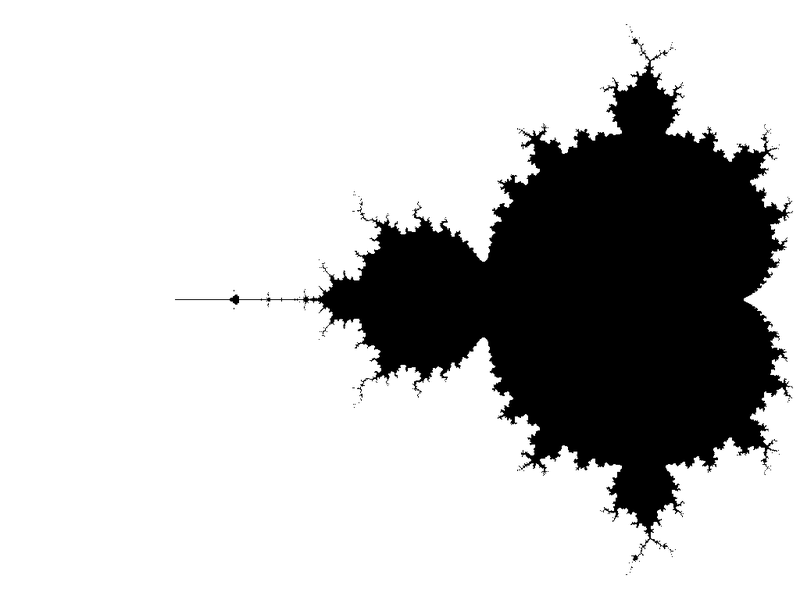
\includegraphics[width=10cm]{img/mandelbrot_b&w.png}
    \centering
    \caption{Two color version of the quadratic Mandelbrot set $z=0$. \cite{mandelbrot_b&w}}
    \label{fig:mandelbrot_b&w}
\end{figure}
\\ \\
This method can be improved by coloring each pixel, whose $p$ is not present in the set using the value of $g(p, c)$. This will uncover a great amount of detail and expose the amazing complexity of the Mandelbrot set - see figure 1.2.

\begin{figure}[ht]
    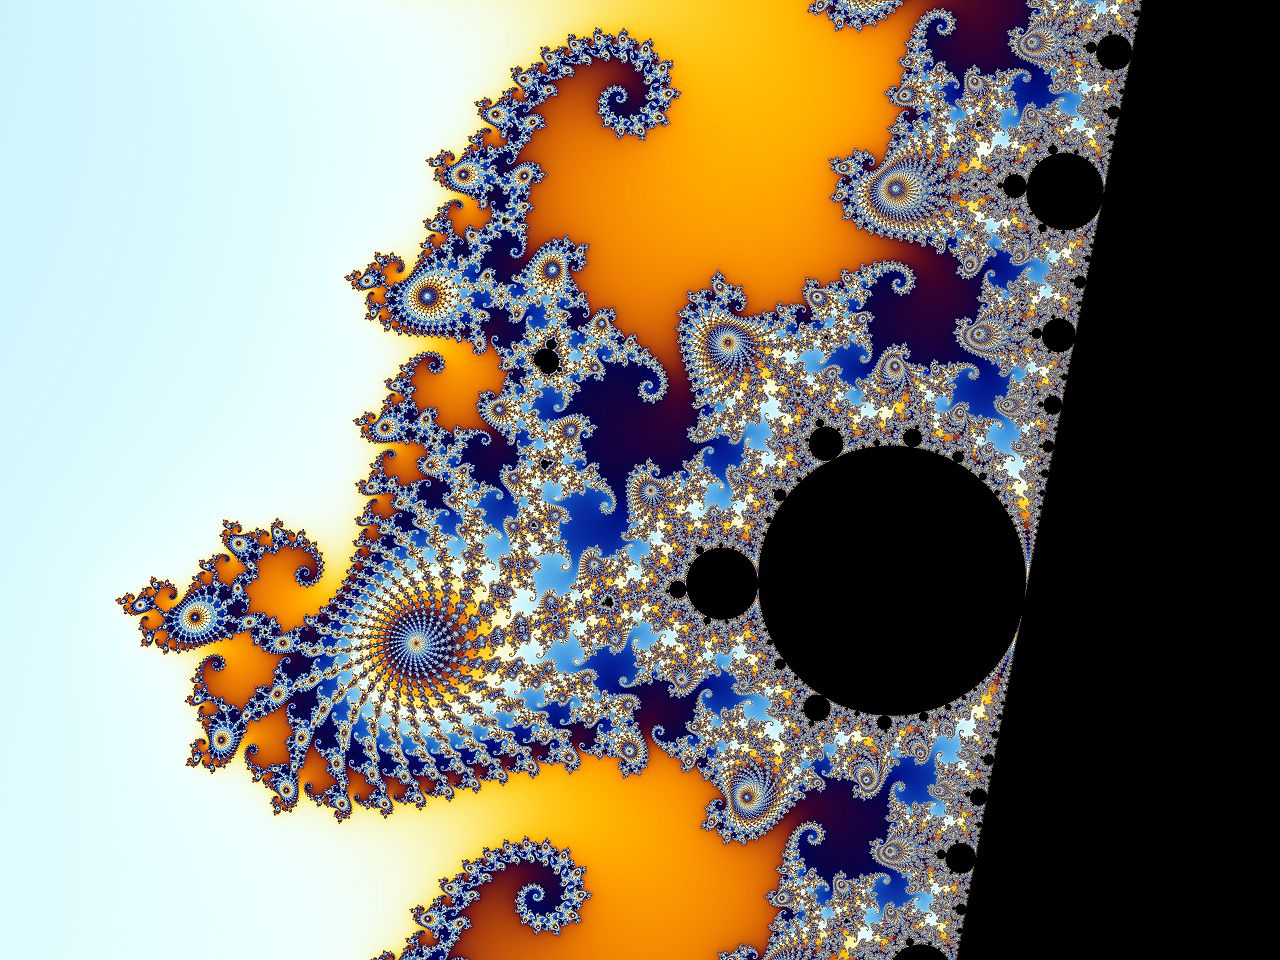
\includegraphics[width=10cm]{img/mandelbrot_color.jpg}
    \centering
    \caption{$M_0$ colored based on the value of $g(p,c)$. \cite{mandelbrot_color}}
    \label{fig:mandelbrot_color}
\end{figure}

\section{Julia Sets Of Quadratic Polynomials}
Julia set of a quadratic polynomial $J_c$ is the set of all $z$ for which $F(z,\:c)$ is bounded.\cite{julia_set_wiki}\cite{julia_set_wolfram} We can visualize $J_c$ analogously to Mandelbrot set, we just use the complex number $p$ associated with the pixel as the fist argument - $F(c, p)$. 

\section{The Connection}
Since the function $F(z,\:c)$ has 2 complex parameters ($z = [z_a, z_b], c = [c_a, c_b]$), we can associate each point in 4-dimensional space $P[z_a, z_b, c_a, c_b]$ with a value of $F(z,\:c)$. Both $M_z$ and $J_c$ are then cross sections of this object. $M_z$ is parallel to the two $z$ axes and $J_c$ to the two $c$ axes. We can, however also plot cross sections of this space that are not parallel to the axes. Our plane is rotated from $z_a$ to $c_a$ with the angel $\alpha$ and from $z_b$ to $c_b$ with the angel $\beta$.
\[F_r(x, y, \alpha, \beta) = F(cos(\alpha)*x, cos(\beta)*y, sin(\alpha)*x, sin(\beta)*y,\]


\chapter{Implementation}
In the second chapter of my Thesis, I will write about the decisions I had to make during the development, why I made the ones I made, If I think they were the right ones and how I would approach the project with the benefit of hindsight.
\section{2-Dimensional slices}
Shortly after turning in the official assignment worksheet, I realized making the slices 3-dimensional was not a good idea. Making 3-dimensional slices of a 4-dimensional object is not more difficult than making 2-dimensional slices. The problem is with rendering them. All of the 3-dimensional slices would have no outside border, many of them would have no inside border either. On top of that, the object I was rendering had a lot of inner complexity, and to expose it, the slices would have to be 2-dimensional.
\section{Unity Post-Processing Shader}
Since this task is computationally difficult - the function $f$ is evaluated up to $R_x * R_y * I_m$ times. I needed to leverage GPU acceleration in order to run the rendering program in real-time. I had some very limited experience with the game engine Unity and I knew it featured shaders - programs that run parallelly on the many GPU cores for every pixel on the screen - so I decided to use it. I rendered an empty scene and added the fractal as a post-processing shader written in High-Level Shading Language. It worked, but it was not an ideal way to approach the problem. Unity post-processing shaders are meant for a very specific use case and were not build to be used this way.
\section{OpenGL Rewrite}
After the first consultation, I decided to rewrite the whole thing using C++ and OpenGL. I was not satisfied with the Unity HLSL documentation and I felt like OpenGL would provide me with more flexibility. While OpenGL has turned out to be more difficult to use than I anticipated, I still believe this was the right decision.
\section{Double-Shader Architecture}
\label{section:ds_architecture}
To show more detail, I wanted the fractal to use the whole color spectrum, even if all the values visible on the screen were very close together. But since the whole point of using a shader is parallelization, it was impossible to know other values on the screen before the whole shader program has finished. And so I had to convert my program architecture into a more complex one. First, in the compute shader I calculate the value of $g(z,c)$ for every pixel on the screen. At this step, I also save the lowest and highest values recorded and save it together with all the values in a Buffer on the GPU. Then in the fragment shader, I color each pixel based on where its associated value lays in the interval from the lowest value to the highest one. I do not believe this would be possible if I carried on with the Unity approach.
\section{Performance Issues}
The OpenGL application runs very slowly on my laptop, which is not surprising - my laptop has no dedicated GPU. But it runs even slower on my PC with GTX 1650. I have spent many hours profiling, debugging, researching, and even posted a question to Stack Overflow. I tried rewriting the application to use different buffers for writing and reading values. In the end, I was not able to improve the performance. 

\section{Mysterious Bugs}
In the development of the application, I have encountered some bugs I just could not wrap my mind around. As an example, I noticed that after moving around in the fractal and stopping, the fractal colors were shivering for a while, then settled. I checked and double-checked every variable involved in the equation that determined the color of every pixel - none of them changed after I stopped touching the keyboard. Yet the colors on the screen changed. After a few hours, I just gave up. I accepted the fractal will keep on shivering from time to time. A week later, I noticed the same shivering when I opened a picture on my computer. The monitor was adjusting it is dynamic range - slowly so it would not be as noticeable. 
\section{The Benefit Of Hindsight}
I have learned a lot in the development process. If you divide the time I have spent on the project by the number of lines of code I have produced, it is by far the most time-dense project of mine. If I were to take on the project today, with the experience I gained in the process, I would approach it very differently. I would choose to create an application that does not run in real-time, but instead saves the rendered images and creates a video of the movement through the fractal. This would be possible to do on the CPU. I would not have to spend so much time navigating technologies I was not at all familiar with and would allow me to invest more time into developing additional features.

\chapter{Technical Documentation}
In the last chapter of my thesis, I will provide information that will allow you to run and use the application.

\section{Running The Application}
First, download \underline{\href{https://github.com/MikulasVanousek/4D-fractal/archive/refs/heads/master.zip}{the code}}. Then extract the archive contents. The archive contains a 4D-fractal-master folder - inside you will find the source code.
\subsection{Windows}
Inside 4D-fractal-master/Windows/Release you will find fractal-cpp.exe. You should be able to run it - if not, see section \ref{section:OpenGL}.
\subsection{Linux And Mac OS}
On operating systems other than Windows, you will have to compile the application yourself. This can be a bit tricky to do, so I will provide you with some guidance.
\begin{itemize}
    \item You might be able to import the solution into visual studio. If you do, you should be able to compile it and run the app that will be created in the Release folder. (You might still have to copy the shader files.) 
    \item If you are not able to import the project, you can create a project from existing code and link all the libraries necessary - GLEW (static version), GLFW, linmath. To link the libraries, go to project properties and do the following:
    \begin{itemize}
        \item Add all the include directories.
        \item Add all the additional library directories (32-bit versions).
        \item Add all the additional dependencies.
        \item Add GLEW\_STATIC preprocessor definition.
        \item For more details see \cite{cherno}.
    \end{itemize}
    \item You also need to make sure the shader files (vs.shader, cs.shader, fr.shader) will be copied to the output directory. This can be done by setting up the IDE to do this for you when the project is compiled or you can do this manually. 
\end{itemize}

\subsection{Installing OpenGL Driver}
\label{section:OpenGL}
For the application to run, you need to have OpenGL 4.5.0 or a newer driver installed on your GPU. If your GPU driver is up to date, OpenGL 4.5.0 should be included. The version of OpenGL installed can be found in the console output of the application. If your version is lower than 4.5.0 or no OpenGL driver is installed, download the newest driver from the website of your GPU manufacturer and follow their installment instructions.

\section{Controls}
The controls work best with QWERTY keyboard layout.
\begin{itemize}
    \item Use \keystroke{D}(+) \keystroke{A}(-) to mover your view along $x$ - the horizontal axis of the slice.
     \item Use \keystroke{W}(+) \keystroke{S}(-) to mover your view along $y$ - the vertical axis of the slice.
    \item Use \keystroke{R}(+) \keystroke{F}(-) to move along $a$ - the first perpendicular axis to the slice.
    \item Use \keystroke{T}(+) \keystroke{G}(-) to move along $b$ - the second perpendicular axis to the screen.
    \item Use \keystroke{Y}(+) \keystroke{H}(-) to rotate the slice $\frac{\pi}{2}$ along the $y$ and $b$ axes - $y$ and $b$ still point in the same direction.
    \item Use \keystroke{U}(+) \keystroke{J}(-) to rotate the slice $\frac{\pi}{2}$ along the $x$ and $a$ axes - $x$ and $a$ still point in the same direction.
    \item Use \keystroke{L-Shift}(+) \keystroke{L-Ctrl}(-) to control zoom.
    \item Use \keystroke{R-Shift}($\times2$) \keystroke{R-Ctrl}($\times \frac{1}{2}$) to control the maximum number of iterations.
    \item Use \keystroke{Esc} to exit the application.
    
\end{itemize}


\chapter*{Conclusion}
\pagestyle{empty}
\addcontentsline{toc}{chapter}{Conclusion}
The original goal of my work was to create a Linux application visualizing 3-d slices of the fractal. Unfortunately, I did not do enough research before writing the specification. I chose a very difficult assignment and therefore even in the midst of my work, I was not sure how it is going to turn out. Due to the severe lack of experience in the field, I had to pivot many times during the development process, which prevented me from fulfilling some of the originally laid out goals. Visualizing 3-dimensional slices turned out not only impractical but borderline impossible. The application was originally meant to be for Linux. When I replaced Ubuntu with Windows on my laptop, I relied on the Unity cross-platform compilation. After the OpenGL rewrite, I lost this option - the application is for Windows only. 

Nevertheless, I believe I succeeded in my goal to visualize the relationship between quadratic Mandelbrot sets and quadratic Julia sets. Rotating the slice of the 4-dimensional function allows the user to see other slices of the fractal than the ones parallel to the axes. This gives the user much more freedom in the exploration of the 4-dimensional object and it allows him to understand how quadratic Mandelbrot sets and quadratic Julia sets are the object's orthogonal slices. 

I gained a lot of experience working on this thesis. I realized how important the initial choice of technologies is and how mistakes in the onset of a project caused by the lack of expertise can be very costly. I also experienced firsthand the complexity associated with programming in the lower abstraction levels and working directly with the hardware. This helped me narrow down the domain of IT I want to specialize in and identify some areas of IT I will try to avoid in the future. 

The performance issues, while agonizing for me, luckily are not severe enough to prevent the user from gaining the insight this thesis is supposed to provide. If I were to take on the project today, with the experience I gained in the process, I would approach it very differently - instead of creating a real-time application running on the GPU, I would use the CPU to render a 60 FPS video of the movement through the fractal. I would not have to spend so much time navigating technologies I was not at all familiar with, which would allow me to invest more time into developing additional features.

 


%%% Seznam použité literatury
\nocite{*}
 \printbibliography[title={Citations},heading={bibintoc}]

%%% Seznam obrázků
%\chapter*{List Of Figures}
%\pagestyle{empty}
%%% TODO List of figures hyperlink
\openright
\pagestyle{empty}
\noindent
\listoffigures
\addcontentsline{toc}{chapter}{List Of Figures}

%%% Seznam tabulek
 
%%% TODO remove EMPTY PAGES

%%%\listoftables
%%%\addcontentsline{toc}{chapter}{Seznam tabulek}

%%% Přílohy k práci, existují-li. Každá příloha musí být alespoň jednou
%%% odkazována z vlastního textu práce. Přílohy se číslují.

%\part*{Přílohy}
%\appendix

\end{document}
